% Licensed under the Creative Commons Attribution Share Alike 4.0 International.
% See the LICENSE file in the repository root for full license text.

\section{实验:手动引用第三方库\label{sec:experiment-2}}

上一节中,我们复习了包含多个源文件的 C++ 程序的生成流程。本节我们将利用上一节的知识,探索手动引用第三方库的方法,规避可能出现的编译错误和链接错误。

\subsection*{实验步骤}

\begin{enumerate}
	\item 新建项目和源文件。操作步骤与 \ref{sec:experiment-1} 相同,项目中只包含 \lstinline[language={}]{main.cpp} 一个文件。

	\item 以源代码的形式引用 JsonCpp 库。\label{item:exp-2-2}

	JsonCpp\footnote{网址:\url{https://github.com/open-source-parsers/jsoncpp}。} 是一个用于解析 JSON 格式文本并操纵 JSON 对象的 C++ 库,而 JSON 是一种常用的数据交换格式,下面是 JSON 格式文本一例。

	\begin{lstlisting}[language={JSON}]
{
	"name": "John Doe",
	"age": 42,
	"phones": [
		{ "type": "home", "number": "555-1234" },
		{ "type": "office", "number": "555-2345" },
		{ "type": "mobile", "number": "555-3456" }
	]
}
	\end{lstlisting}

	\begin{enumerate}
		\item 下载源代码。前往 JsonCpp 最新版本的发布页面\footnote{网址:\url{https://github.com/open-source-parsers/jsoncpp/releases/tag/1.9.5}。}下载源码:\url{https://github.com/open-source-parsers/jsoncpp/archive/refs/tags/1.9.5.zip}。解压后,将其中的 \lstinline[language={}]{src} 文件夹和 \lstinline[language={}]{include} 文件夹移动到项目根目录下新建的 \lstinline[language={}]{JsonCpp} 文件夹中。

		\item 将源文件添加到项目中。\label{item:exp-2-2-2}在 Dev-C++ 中打开新建的项目,在“项目管理”窗口中右键点击项目,点击弹出菜单中的“添加文件夹”,命名为“JsonCpp”。在“项目管理”窗口中右键点击刚才新建的“JsonCpp”文件夹,点击弹出菜单中的“添加”,进入项目目录下的 \lstinline[language={}]{JsonCpp/src/lib_json},选择其中所有以 \lstinline[language={}]{.cpp} 为扩展名的文件,点击“打开”。完成后的“项目管理”窗口如图 \ref{fig:manual-library-1} 所示。

		\begin{figure}
			\centering
			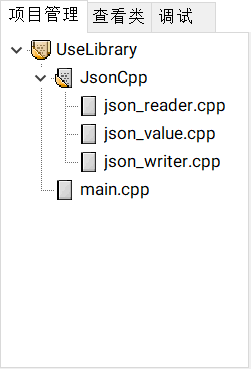
\includegraphics[width=0.2\linewidth]{assets/manual-library-1}
			\caption{添加源文件后的“项目管理”窗口。}
			\label{fig:manual-library-1}
		\end{figure}

		\item 将包含目录添加到项目中。\label{item:exp-2-2-3}在“项目管理”窗口中右键点击项目,点击弹出菜单中的“项目属性”。在弹出的对话框中,点击“文件/目录”选项卡,再点击“包含文件目录”子选项卡。点击右下角的选择文件夹按钮(图 \ref{fig:manual-library-2} 中的蓝色按钮),选择项目目录下的 \lstinline[language={}]{JsonCpp/include} 文件夹,按钮旁的编辑框将显示完整路径。删除其中的绝对路径,只保留 \lstinline[language={}]{JsonCpp/include},然后点击“添加”。完成后的“项目属性”对话框如图 \ref{fig:manual-library-3} 所示\footnote{也可以直接在编辑框中输入 \lstinline[language={}]{JsonCpp/include},不点击选择文件夹按钮。}。最后点击“确定”退出该对话框。

		\begin{figure}
			\centering
			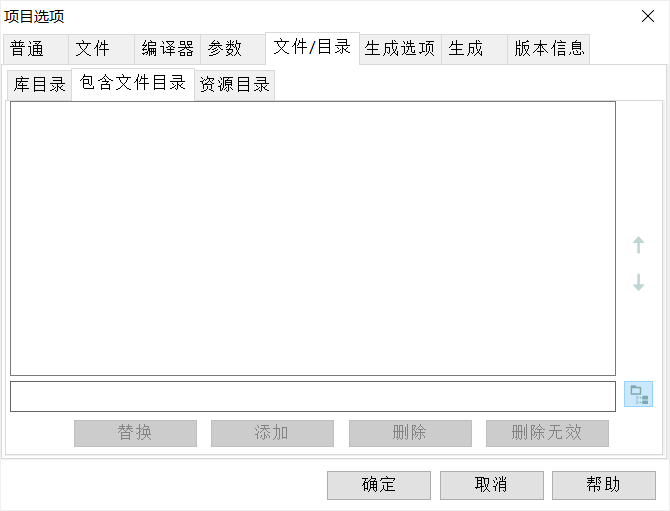
\includegraphics[width=0.75\linewidth]{assets/manual-library-2}
			\caption{“项目属性”对话框。}
			\label{fig:manual-library-2}
		\end{figure}

		\begin{figure}
			\centering
			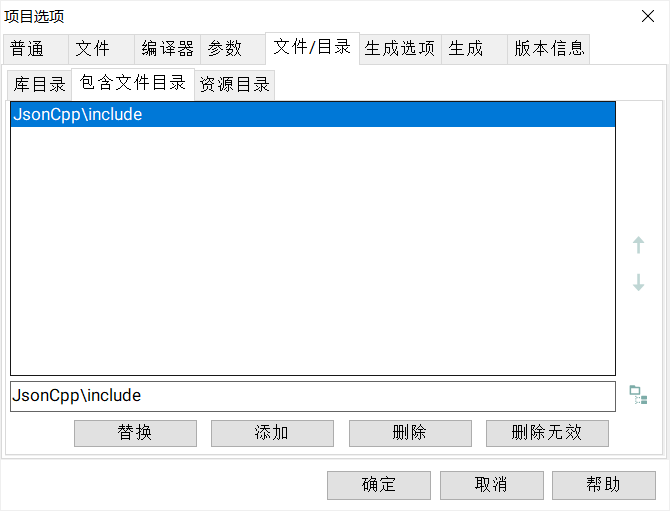
\includegraphics[width=0.75\linewidth]{assets/manual-library-3}
			\caption{完成后的“项目属性”对话框。}
			\label{fig:manual-library-3}
		\end{figure}

		\item 编写代码。

		\begin{lstlisting}[language={[17]C++}, moreemph={[1]Value}]
// main.cpp
#include <json/json.h>

int main()
{
	Json::Value v = 1;
}
	\end{lstlisting}

		\item 编译并运行代码。“编译日志”窗口记录的命令如下。

		\begin{lstlisting}[language={}]
g++.exe -c main.cpp -o main.o -I"Dev-Cpp/TDM-GCC-64/include" -I"JsonCpp/include"

g++.exe -c JsonCpp/src/lib_json/json_reader.cpp -o JsonCpp/src/lib_json/json_reader.o -I"Dev-Cpp/TDM-GCC-64/include" -I"JsonCpp/include"

g++.exe -c JsonCpp/src/lib_json/json_value.cpp -o JsonCpp/src/lib_json/json_value.o -I"Dev-Cpp/TDM-GCC-64/include" -I"JsonCpp/include"

g++.exe -c JsonCpp/src/lib_json/json_writer.cpp -o JsonCpp/src/lib_json/json_writer.o -I"Dev-Cpp/TDM-GCC-64/include" -I"JsonCpp/include"

g++.exe main.o JsonCpp/src/lib_json/json_reader.o JsonCpp/src/lib_json/json_value.o JsonCpp/src/lib_json/json_writer.o -o UseLibrary.exe -L"Dev-Cpp/TDM-GCC-64/lib" -static-libgcc
		\end{lstlisting}
	\end{enumerate}

	\item 以二进制的形式引用 SFML 库。\label{item:exp-2-3}

	SFML\footnote{网址:\url{https://www.sfml-dev.org/}。} 全称 Simple and Fast Multimedia Library,是一个用于编写游戏和多媒体应用程序的多媒体库。一般而言,多媒体库较为复杂,从源码构建需要较长的时间,所以下面我们将以二进制的形式引用 SFML 库。

	\begin{enumerate}
		\item 下载源代码和二进制文件。前往 SFML 的代码仓库\footnote{网址:\url{https://github.com/SFML/SFML}。},在最新版本的发布页面\footnote{网址:\url{https://github.com/SFML/SFML/releases/tag/2.5.1}。}下载发布的文件:\url{https://github.com/SFML/SFML/releases/download/2.5.1/SFML-2.5.1-windows-gcc-7.3.0-mingw-64-bit.zip}。注意,此处要选择与你使用的编译器相匹配的版本。将整个 \lstinline[language={}]{SFML-2.5.1} 文件解压到项目根目录下。

		\item 将包含目录添加到项目中。操作步骤与此前相同,添加的包含目录为 \lstinline[language={}]{SFML-2.5.1/include}。完成后的“项目属性”对话框如图 \ref{fig:manual-library-4} 所示。

		\begin{figure}
			\centering
			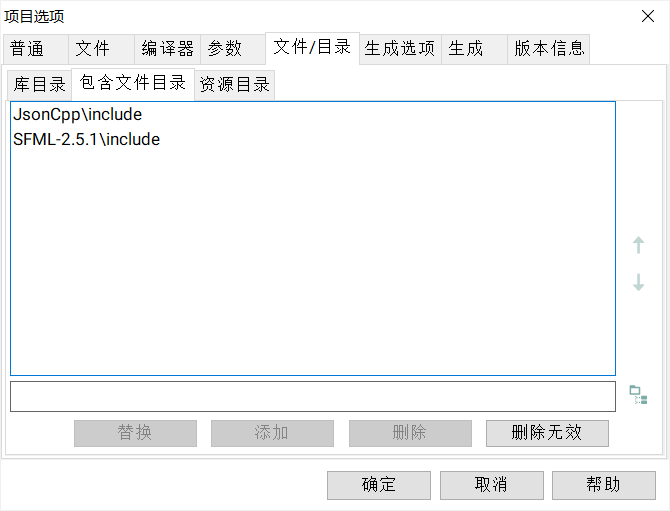
\includegraphics[width=0.75\linewidth]{assets/manual-library-4}
			\caption{添加包含目录后的“项目属性”对话框。}
			\label{fig:manual-library-4}
		\end{figure}

		\item 将附加链接库添加到项目中。\label{item:exp-2-3-3}在“项目属性”对话框中,进入“参数”选项卡,点击“链接”文本框下的“加入库或者对象”,选择项目目录下 \lstinline[language={}]{SFML-2.5.1/lib} 中所有扩展名为 \lstinline[language={}]{.a} 的文件。完成后的“项目属性”对话框如图 \ref{fig:manual-library-5} 所示。

		\begin{figure}
			\centering
			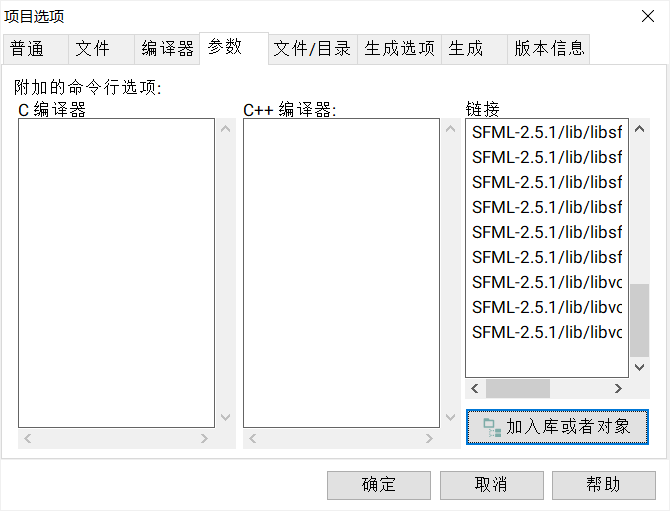
\includegraphics[width=0.75\linewidth]{assets/manual-library-5}
			\caption{添加附加链接库后的“项目属性”对话框。}
			\label{fig:manual-library-5}
		\end{figure}

		\item 编写代码。

		\begin{lstlisting}[language={[17]C++}, moreemph={[1]Value, Window, VideoMode, Event}, moreemph={[2]isOpen, pollEvent, close, display}]
// main.cpp
#include <json/json.h>
#include <SFML/Window.hpp>

int main()
{
	Json::Value v = 1;
	sf::Window window(sf::VideoMode(640, 480), "Hello, world!");
	while (window.isOpen())
	{
		sf::Event event;
		while (window.pollEvent(event))
		{
			if (event.type == sf::Event::Closed)
				window.close();
		}
		window.display();
	}
}
		\end{lstlisting}

		\item 编译代码。“编译日志”窗口记录的命令如下(第 3 行的命令是节选)。

		\begin{lstlisting}[language={}]
g++.exe -c main.cpp -o main.o -I"Dev-Cpp/TDM-GCC-64/include" -I"JsonCpp/include" -I"SFML-2.5.1/include"

g++.exe main.o JsonCpp/src/lib_json/json_reader.o JsonCpp/src/lib_json/json_value.o JsonCpp/src/lib_json/json_writer.o -o UseLibrary.exe -L"Dev-Cpp/TDM-GCC-64/lib" -static-libgcc SFML-2.5.1/lib/libFLAC.a SFML-2.5.1/lib/libfreetype.a ...
		\end{lstlisting}

		\item 将动态链接库拷贝到可执行文件所在目录。\label{item:exp-2-3-6}将 \lstinline[language={}]{SFML/bin} 中所有的 \lstinline[language={}]{.dll} 文件拷贝到项目根目录中,保证生成的 \lstinline[language={}]{.exe} 文件与这些 \lstinline[language={}]{.dll} 文件位于同一目录,如图 \ref{fig:manual-library-6} 所示。

		\begin{figure}
			\centering
			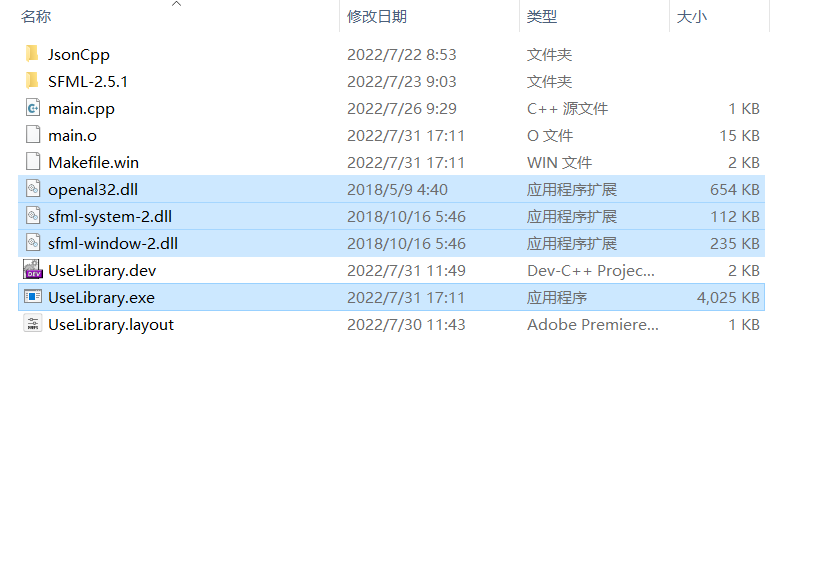
\includegraphics[width=0.75\linewidth]{assets/manual-library-6}
			\caption{需要保证所有 \lstinline[language={}]{.dll} 文件与 \lstinline[language={}]{.exe} 文件位于同一目录。}
			\label{fig:manual-library-6}
		\end{figure}

		\item 运行程序。在 Dev-C++ 中点击菜单栏中的“运行”、“运行”,可以看到一个控制台窗口和一个黑色窗口弹出,如图 \ref{fig:manual-library-7} 所示。

		\begin{figure}
			\centering
			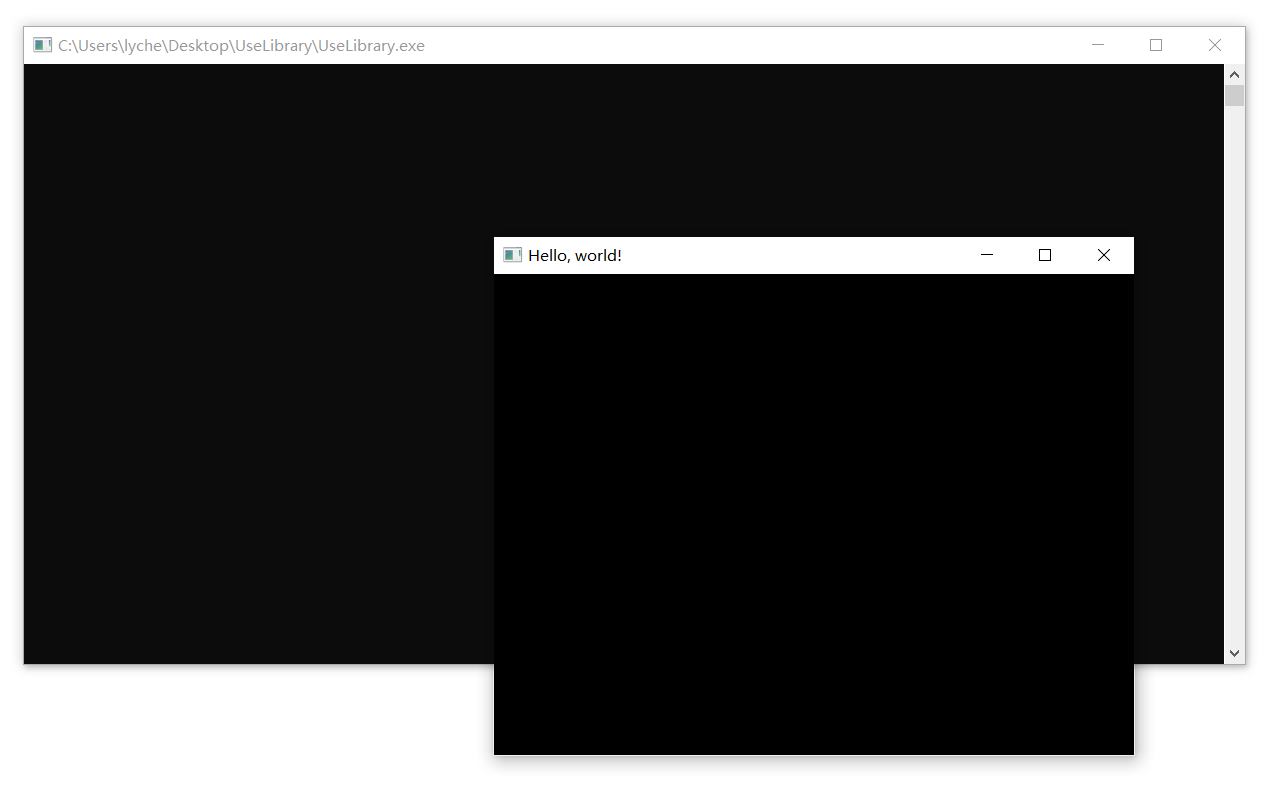
\includegraphics[width=0.75\linewidth]{assets/manual-library-7}
			\caption{程序运行结果。}
			\label{fig:manual-library-7}
		\end{figure}
	\end{enumerate}
\end{enumerate}

\subsection*{讨论}

\begin{enumerate}
	\item 各实验步骤的作用。

	严格按照以上实验步骤进行操作,最终可以得到一个可正常运行的 \lstinline[language={}]{.exe} 文件;而缺失步骤则会导致失败,并且缺失不同的步骤会产生不同的现象。下面我们将讨论这些现象。

	\begin{enumerate}
		\item 不将源文件添加到项目中。

		在第 \ref{item:exp-2-2} 步中,不做第 \ref{item:exp-2-2-2} 小步,编译代码,将得到以下编译日志。

		\begin{lstlisting}[language={}]
g++.exe -c main.cpp -o main.o -I"Dev-Cpp/TDM-GCC-64/include" -I"JsonCpp/include"

g++.exe main.o -o UseLibraryWrong.exe -L"Dev-Cpp/TDM-GCC-64/lib" -static-libgcc

ld.exe: main.o:main.cpp:(.text+0x1a): undefined reference to `Json::Value::Value(int)'

ld.exe: main.o:main.cpp:(.text+0x26): undefined reference to `Json::Value::~Value()'
collect2.exe: error: ld returned 1 exit status
UseLibraryWrong\Makefile.win:25: recipe for target 'UseLibraryWrong.exe' failed
mingw32-make.exe: *** [UseLibraryWrong.exe] Error 1
		\end{lstlisting}

		可以看到,第 1 行的编译命令没有输出其他内容,说明该命令执行成功。而第 3 行的链接命令之后出现了错误信息,且关键在第 5 行和第 7 行;错误信息反馈,在链接时 \lstinline[language={[17]C++}, moreemph={[1]Value}]{Value} 的构造函数和析构函数出现了 “undefined reference to ...” 的情况,这是因为我们没有将这两个函数的实现所在的源文件添加到项目中,导致这两个函数没有出现在链接所需的中间文件内,因此链接器就告诉我们这两个函数的未定义。

		综上,将源文件添加到项目中的作用是保证源文件参与编译,生成对应的中间文件供链接使用。

		\item 不将包含目录添加到项目中。

		在第 \ref{item:exp-2-2} 步中,不做第 \ref{item:exp-2-2-3} 小步,编译代码,将得到以下编译日志。

		\begin{lstlisting}[language={}]
g++.exe -c main.cpp -o main.o -I"Dev-Cpp/TDM-GCC-64/include"

main.cpp:1:10: fatal error: json/json.h: No such file or directory
    1 | #include <json/json.h>
      |          ^~~~~~~~~~~~~
compilation terminated.

UseLibraryWrong\Makefile.win:28: recipe for target 'main.o' failed
mingw32-make.exe: *** [main.o] Error 1
		\end{lstlisting}

		编译日志的第 3 行反馈,在编译 \lstinline[language={}]{main.cpp} 时就发生了错误,无法找到路径为 \lstinline[language={}]{json/json.h} 的文件。这是因为该路径是一个相对路径,但我们没有通过额外包含目录告诉编译器基础路径,因此编译器无法找到该文件。

		综上,将包含目录添加到项目中的作用是保证 \lstinline[language={[17]C++}]{#include} 指令知道相对路径对应的基础路径,从而顺利找到要包含的头文件。

		\item 不将附加链接库添加到项目中。

		在第 \ref{item:exp-2-3} 步中,不做第 \ref{item:exp-2-3-3} 小步,编译代码,将得到以下编译日志(节选)。

		\begin{lstlisting}[language={}]
g++.exe main.o JsonCpp/src/lib_json/json_reader.o JsonCpp/src/lib_json/json_value.o JsonCpp/src/lib_json/json_writer.o -o UseLibraryWrong.exe -L"Dev-Cpp/TDM-GCC-64/lib" -static-libgcc

ld.exe: main.o:main.cpp:(.text+0xb2): undefined reference to `__imp__ZN2sf9VideoModeC1Ejjj'

ld.exe: main.o:main.cpp:(.text+0x118): undefined reference to `__imp__ZNK2sf6Window6isOpenEv'

collect2.exe: error: ld returned 1 exit status
UseLibraryWrong\Makefile.win:25: recipe for target 'UseLibraryWrong.exe' failed

mingw32-make.exe: *** [UseLibraryWrong.exe] Error 1
		\end{lstlisting}

		此处的现象与不将源文件添加到项目中的现象相同,都出现了“undefined reference to ...”的错误信息。事实上,附加链接库就是一种编译产生的中间文件,其中包含了函数实现的编译结果。将附加链接库添加到项目中的作用是保证这些中间文件参与链接。

		\item 不将动态链接库拷贝到可执行文件所在目录。

		在第 \ref{item:exp-2-3} 步中,不做第 \ref{item:exp-2-3-6} 小步,编译代码,发现没有出现错误。通过 Dev-C++ 运行程序却无法正常运行,如图 \ref{fig:manual-library-8} 所示。在文件资源管理器中双击打开 \lstinline[language={}]{.exe} 文件,会弹出图 \ref{fig:manual-library-9} 所示的对话框,提示找不到 \lstinline[language={}]{.dll} 文件。

		\begin{figure}
			\centering
			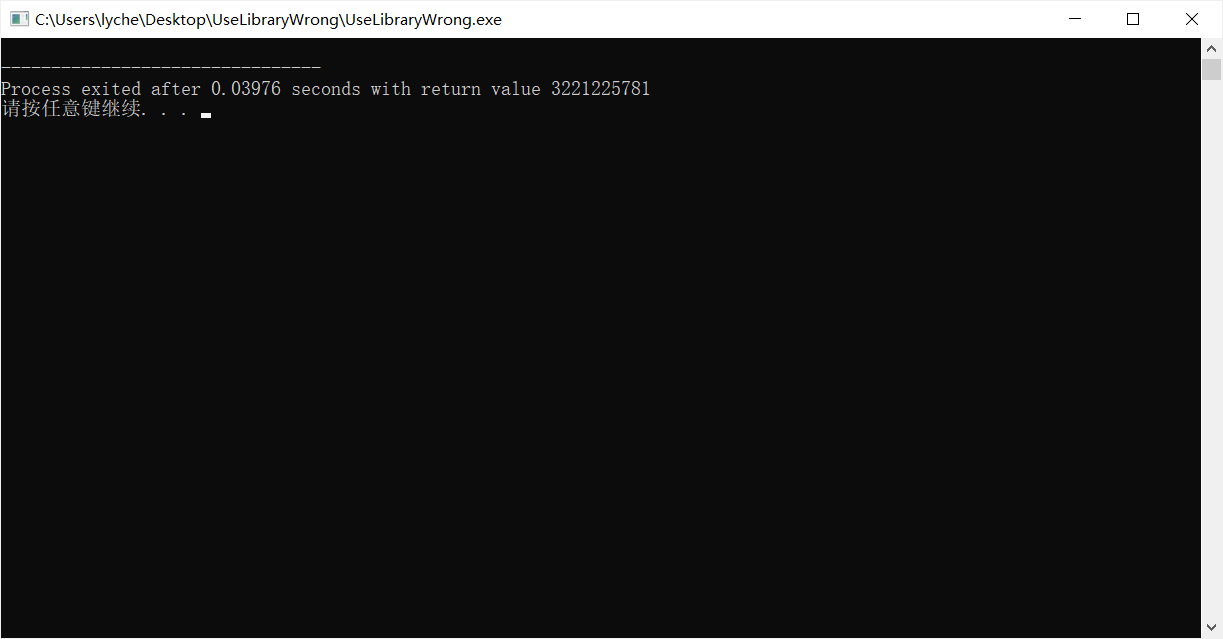
\includegraphics[width=\linewidth]{assets/manual-library-8}
			\caption{返回值非零说明程序异常退出。}
			\label{fig:manual-library-8}
		\end{figure}

		\begin{figure}
			\centering
			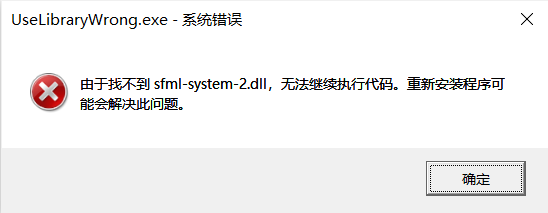
\includegraphics[width=0.75\linewidth]{assets/manual-library-9}
			\caption{无法找到 \lstinline[language={}]{.dll} 文件的错误提示框。}
			\label{fig:manual-library-9}
		\end{figure}

		事实上,DLL 即\emph{动态链接库(Dynamic Linking Library)}的缩写,而动态链接指在运行时动态加载包含可执行代码的 DLL 文件,有别于此前在生成时将代码链接到可执行文件中的过程。因为动态链接库是单独的文件,不同程序可以共用同一个动态链接库,所以通用的函数常以动态链接的形式使用,以减小可执行文件的大小。

		综上,将动态链接库拷贝到可执行文件所在目录的作用是保证程序在运行时可以找到需要动态加载的文件。
	\end{enumerate}

	\item 使用相对路径的作用。添加包含目录到项目中时,尽管选择文件夹对话框为我们生成了绝对路径,但我们只保留了其中的相对路径。这样做的目的是保证项目文件夹被移动到其他位置后仍能正常进行生成;如果使用绝对路径,移动项目文件夹后就无法找到添加的包含目录了。

	\item 编写以上样例代码的目的。

	在第 \ref{item:exp-2-2} 步编写代码时,我们只简单写了 \lstinline[language={[17]C++}, moreemph={[1]Value}]{Json::Value v = 1;} 一句代码,这个程序没有输入输出,也没有任何意义。为什么不写一个具有简单输入输出的样例程序,或者干脆不写?

	编写以上样例代码的目的其实是测试是否成功引用第三方库,所以不必编写一个具有实际意义的程序。但如果不编写任何调用第三方库函数的代码,链接器就不会在中间文件中查找任何第三方库的函数,也就无法起到检查是否成功引用第三方库的作用。

	\item 不同编译器的编译日志。

	不同编译器的编译日志是大同小异的,例如,“undefined reference to ...” 错误在 MSVC 编译器中具有如下形式。

	\begin{lstlisting}[language={}]
main.obj : error LNK2019: 无法解析的外部符号 "void __cdecl foo(void)" (?foo@@YAXXZ),函数 main 中引用了该符号
	\end{lstlisting}

	尽管不同编译器有不同的中间文件格式、不同的错误代码、不同的提示语言,但所有编译器的原理都是一样的,读者应该主动根据编译器报出的错误信息排查上文涉及的错误。

	\item 附加链接目录。

	图 \ref{fig:manual-library-3} 所示的“文件/目录”选项卡中,还有一个“库目录”子选项卡,为什么我们配置外部库时没有用上它?从图 \ref{fig:manual-library-5} 中链接库的路径可以看出,因为我们已经为中间文件指定了完整的相对路径(\lstinline[language={}]{SFML-2.5.1/lib/}),所以无需再通过“库目录”进行指定。

	不过,我们自然不希望重复写多次相对路径,我们可以尝试执行以下步骤。

	\begin{enumerate}
		\item 删除图 \ref{fig:manual-library-5} “参数”选项卡的“链接”文本框中的所有基础路径 \lstinline[language={}]{SFML-2.5.1/lib/}。
		\item 在“文件/目录”选项卡的“库目录”子选项卡中,添加路径 \lstinline[language={}]{SFML-2.5.1/lib}。
	\end{enumerate}

	删除编译好的可执行文件,重新编译,却发现出现如下错误(节选)。

	\begin{lstlisting}[language={}]
g++.exe: error: libFLAC.a: No such file or directory
g++.exe: error: libfreetype.a: No such file or directory
	\end{lstlisting}

	这似乎说明我们添加的库目录没有起作用。事实上,链接外部库应该使用编译选项 \lstinline[language={}]{-l},且无需以 \lstinline[language={}]{lib} 开头、无需指定扩展名。例如,我们需要把“链接”文本框中的 \lstinline[language={}]{libFLAC.a} 修改为 \lstinline[language={}]{-lFLAC}。像前文那样直接写中间文件路径并不是标准的链接外部库的方式,那种写法应当只用于刚刚编译好的中间文件的链接;\textbf{使用 \lstinline[language={}]{-L} 指定的附加链接目录只对使用 \lstinline[language={}]{-l} 选项指定的库有效}也印证了这一观点。

	\item 适用于调试的库文件。
\end{enumerate}
